%        File: HW2.tex
%     Created: Tue Feb 22 09:00 AM 2011 C
% Last Change: Tue Feb 22 09:00 AM 2011 C
%
\documentclass[letterpaper]{article}
\usepackage{amsmath,amsfonts}
\usepackage[margin=.75in]{geometry}
\usepackage[]{graphicx}
\usepackage{listings}
\usepackage{color}
\usepackage{textcomp}
\definecolor{listinggray}{gray}{0.9}
\definecolor{lbcolor}{rgb}{0.9,0.9,0.9}
\lstset{
	backgroundcolor=\color{lbcolor},
	tabsize=4,
	rulecolor=,
	language=Python,
        basicstyle=\scriptsize,
        upquote=true,
        aboveskip={1.5\baselineskip},
        columns=fixed,
        showstringspaces=false,
        extendedchars=true,
        breaklines=true,
        prebreak = \raisebox{0ex}[0ex][0ex]{\ensuremath{\hookleftarrow}},
        frame=single,
        showtabs=false,
        showspaces=false,
        showstringspaces=false,
        identifierstyle=\ttfamily,
        keywordstyle=\color[rgb]{0,0,1},
        commentstyle=\color[rgb]{0.133,0.545,0.133},
        stringstyle=\color[rgb]{0.627,0.126,0.941},
}
\addtolength{\parskip}{\baselineskip}

\title{Statistical Mechanics: HW 5}
\author{Truman Ellis}

\begin{document}
\maketitle

We use the Verlet algorithm to integrate the equations of motion of a single particle of mass
$m=1$ moving on the Muller potential. I start our simulations at the lowest
energy potential, which I found at $(x,y) = (-0.5582, 1.4417)$ which had a
Muller potential of $-146.7$. I randomly set the initial velocity direction, but
fix the magnitude to give a total energy of either $-39$ or $-45$. I found that
a timestep of $\Delta t=4\times10^{-3}$ consistently gave an energy error of less
than one percent and that 200,000 timesteps allowed the simulation to reach an
equilibrium average for $x$, $y$, and $xy$. 

The particle with a total energy of $E=-39$ had enough kinetic energy to
occasionally break out of the deepest energy well and explore some other part of
the domain. When it did, it always got caught in a neighboring well for some
time before breaking out of that one and reentering the original well. I would
let this process repeat a sufficient number of times until a reliable average
could be calculated. In most cases, however, there was sufficient symmetry in the problem
for the particle to follow a repeating path in which it never broke out of the
energy well. Several sample trajectories are illustrated in Figures (1) - (7).
The particle with total energy $E=-45$ never had enough kinetic
energy to break out of the energy potential barrier, and thus never got to
explore other parts of the problem domain. In each run, it would just achieve
some path symmetry and repeat this pattern until the end of the simulation.
There appeared to be fewer trajectory patterns for this lower energy particle.
Figures (8) - (11) illustrate several sample patterns.

We would expect that for a given energy, the expected $x$, $y$, and $xy$ values
would be the same no matter which starting point and which direction the initial
velocity was directed towards, but as the plots demonstrate, this is not true.
Even though each simulation originates at the same point, a simple matter of
reorienting the initial velocity vector changes the calculated averages,
sometimes dramatically. I believe this is primarily because the particle gets
stuck in a pattern and never fully explores the approximation space as it
should. Thus, molecular dynamics does not appear to be an adequate solution for
calculating micro-canonical averages. Perhaps if many particles were initialized
at random points in the domain with random velocity orientations, we would do
better. I think a much more efficient approach would be to use some sort of
Monte Carlo technique. This would break the symmetry in the particle paths and
allow a particle to more fully explore the problem space. 

\begin{figure}[p]
\begin{center}
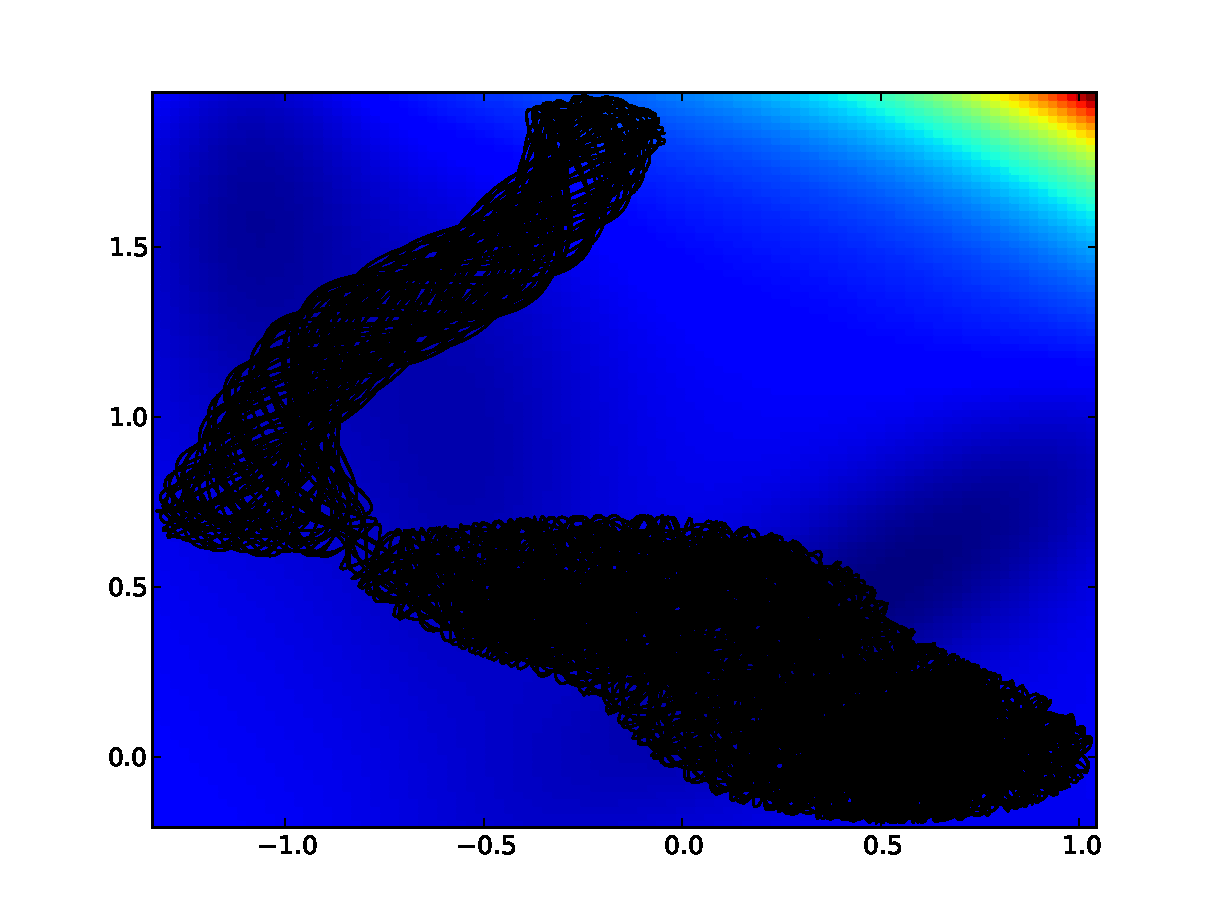
\includegraphics[width=5in]{t1.pdf}
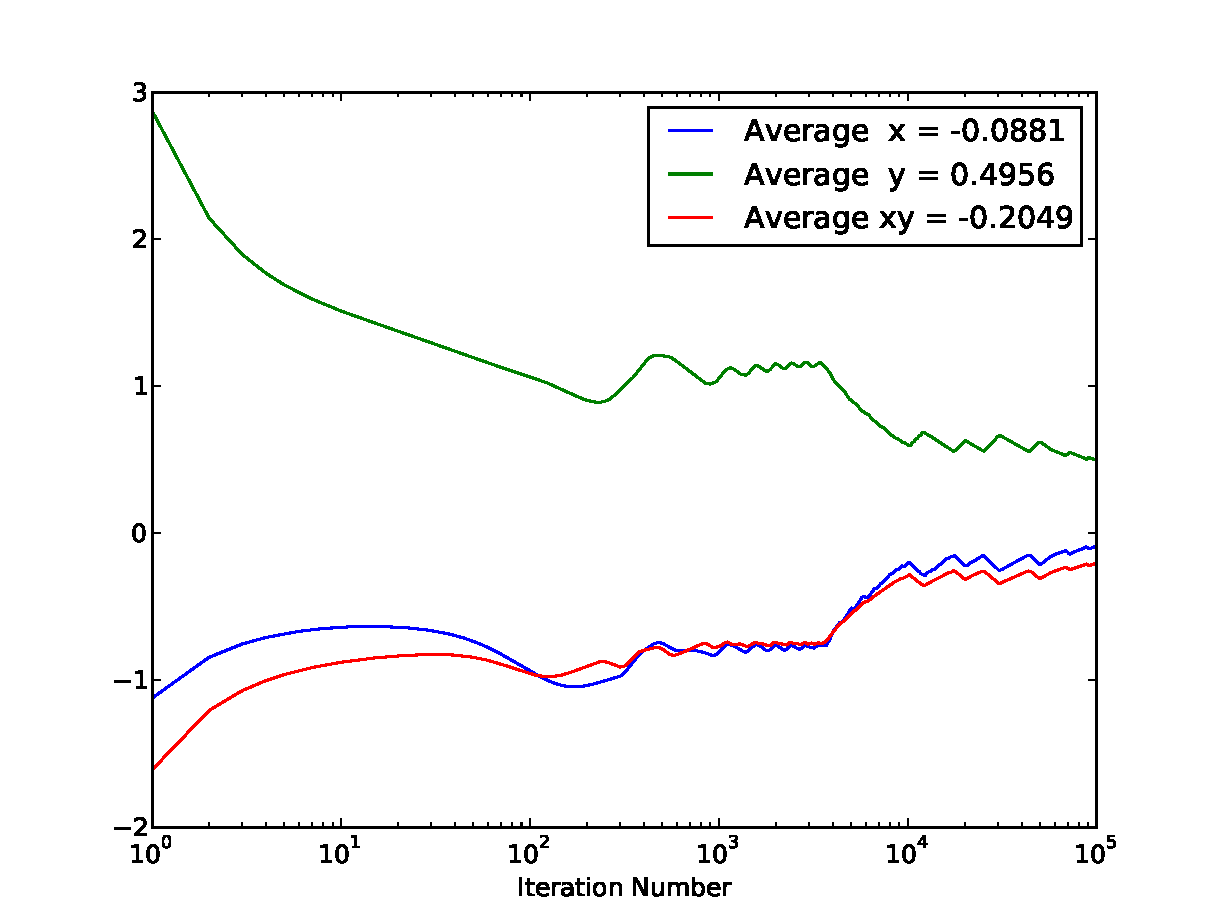
\includegraphics[width=5in]{t1a.pdf}
\end{center}
\caption{$E=-39$: Simulation with 100,000 smaller timesteps $\Delta
t=1\times10^{-3}$ to illustrate
particle path. The plot of the averages does not quite look sufficiently
stabilized in the simulation.}
\label{fig:t1}
\end{figure}

\begin{figure}[p]
\begin{center}
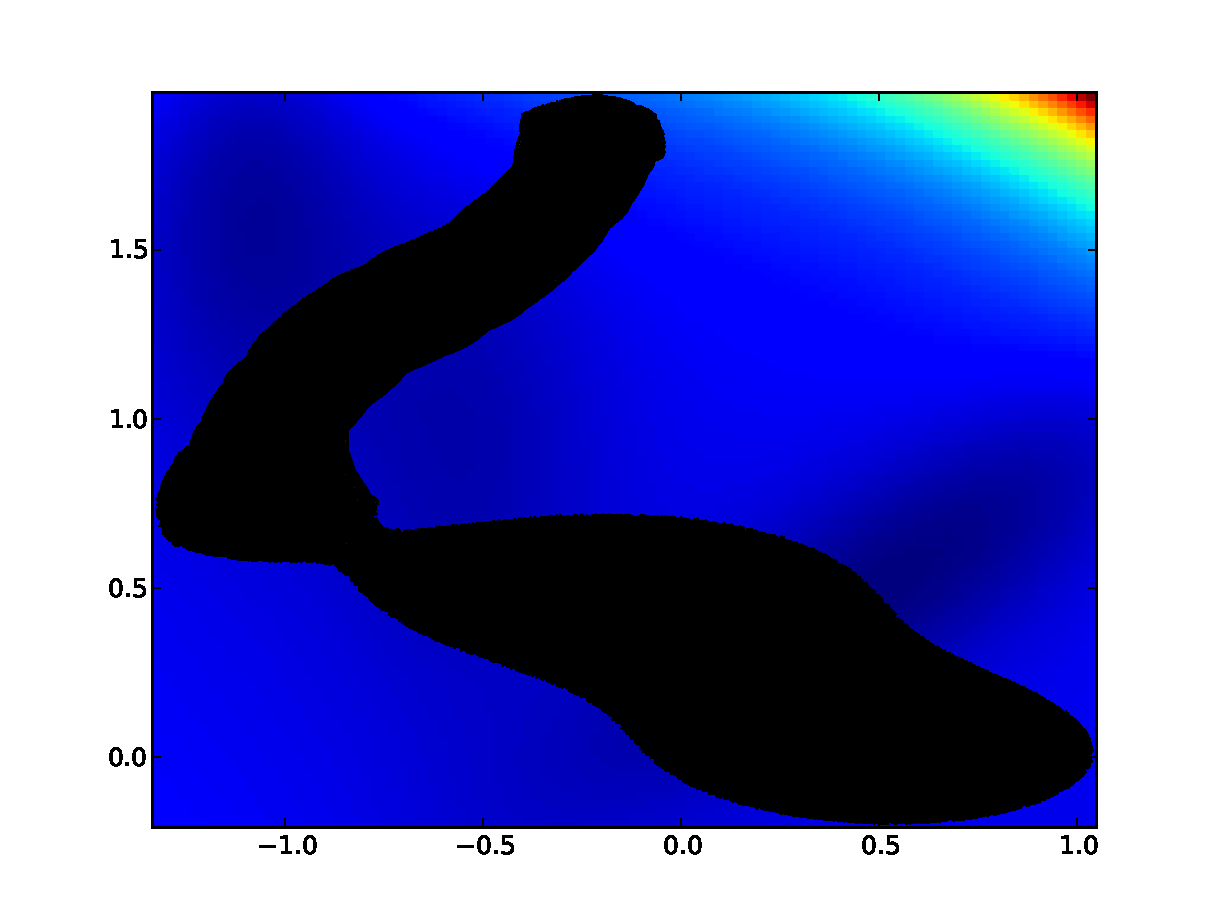
\includegraphics[width=5in]{t5.pdf}
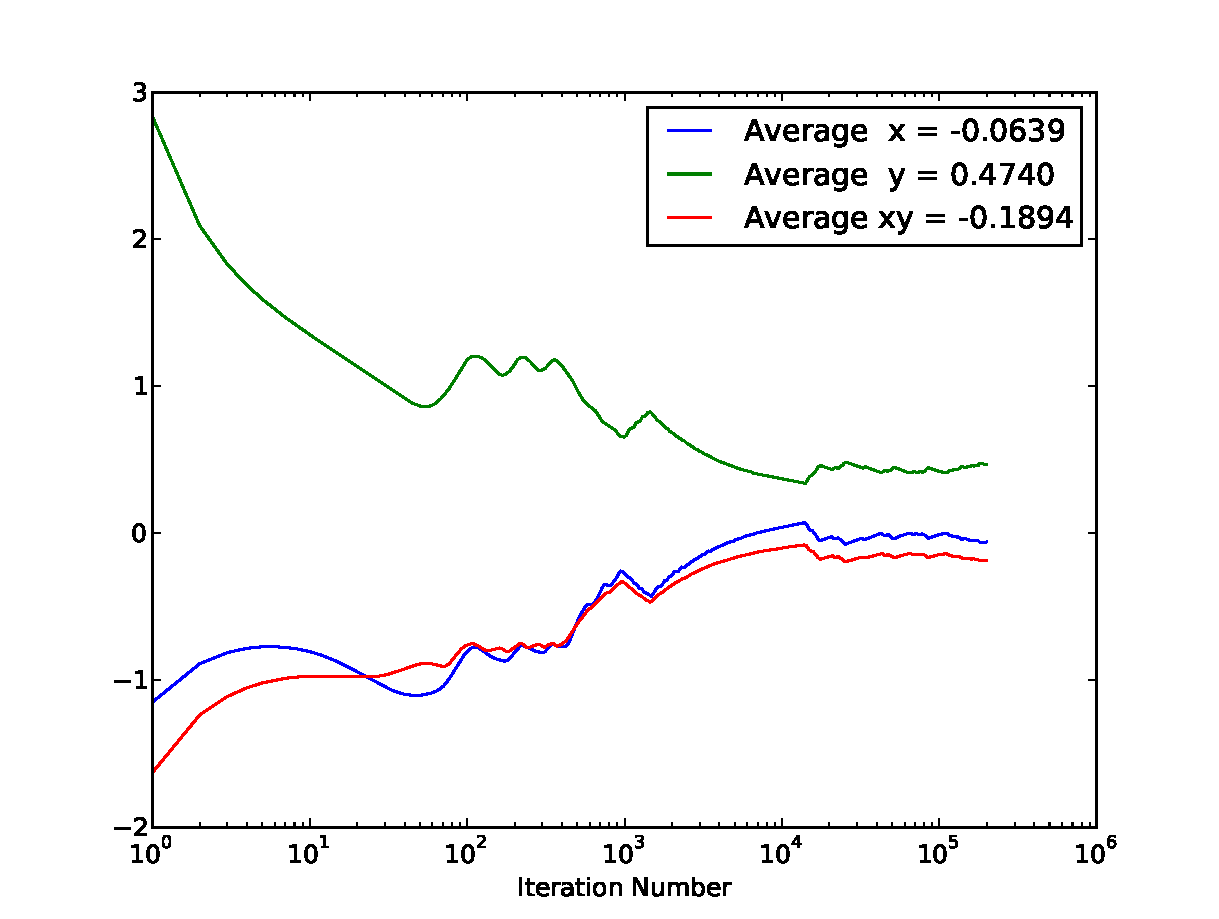
\includegraphics[width=5in]{t5a.pdf}
\end{center}
\caption{$E=-39$: Similar simulation with 200,000 simulations and a larger
timestep. The plot of averages appears to have come to equilibrium. The particle
has covered the space much more efficiently than the previous simulation.}
\label{fig:t5}
\end{figure}

\begin{figure}[p]
\begin{center}
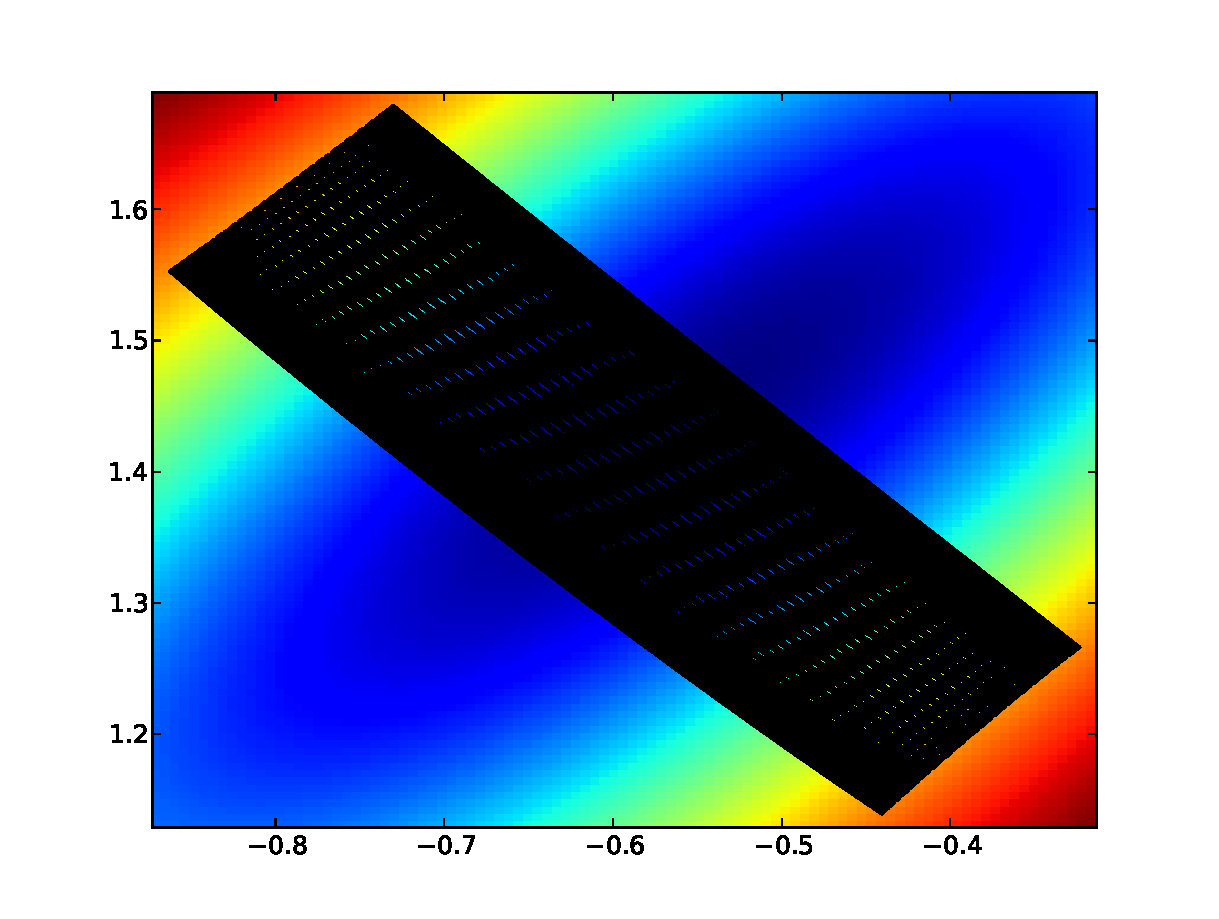
\includegraphics[width=5in]{t8.pdf}
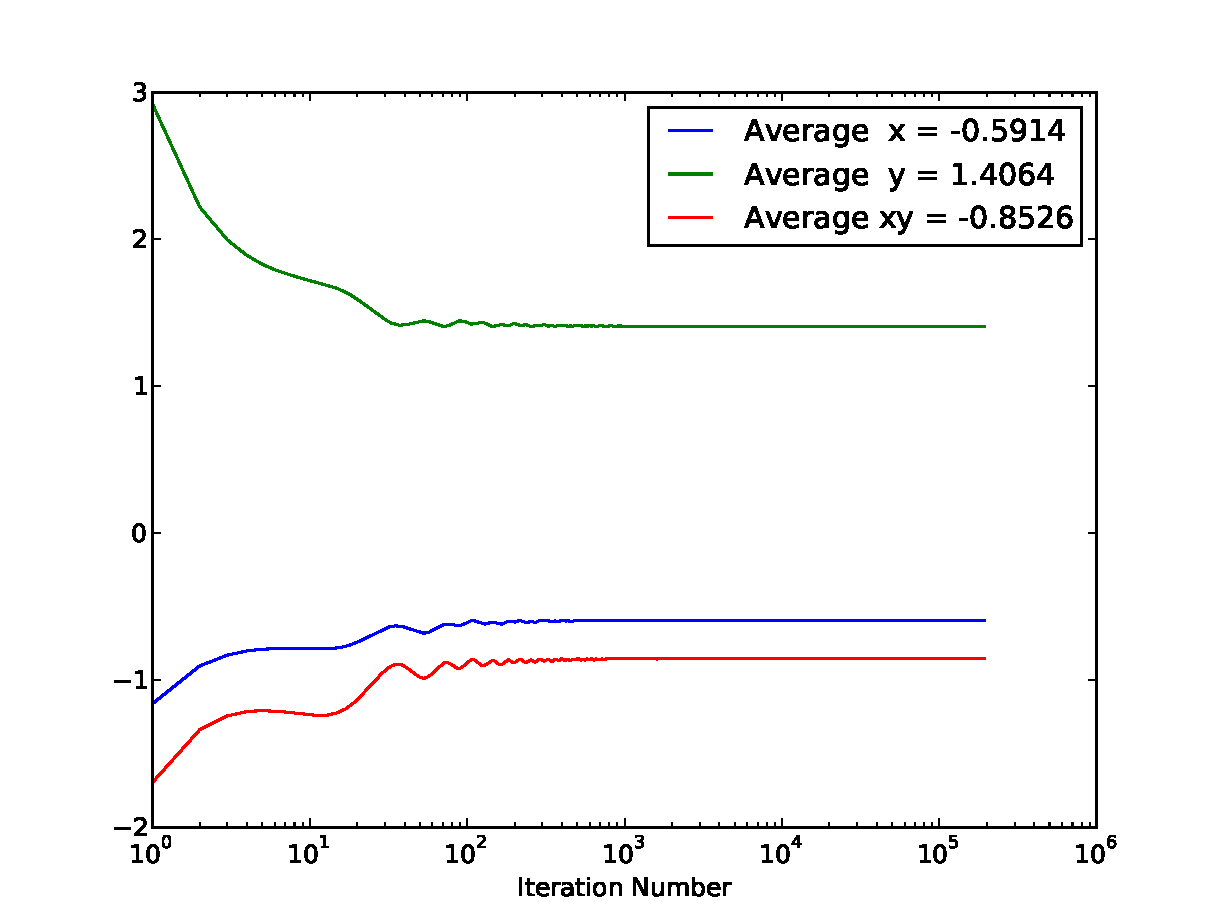
\includegraphics[width=5in]{t8a.pdf}
\end{center}
\caption{$E=-39$: Sometimes the particle finds symmetries in the potential field
and ends up repeating the same path over and over. The small gaps in the path
demonstrate this here.}
\label{fig:t8}
\end{figure}

\begin{figure}[p]
\begin{center}
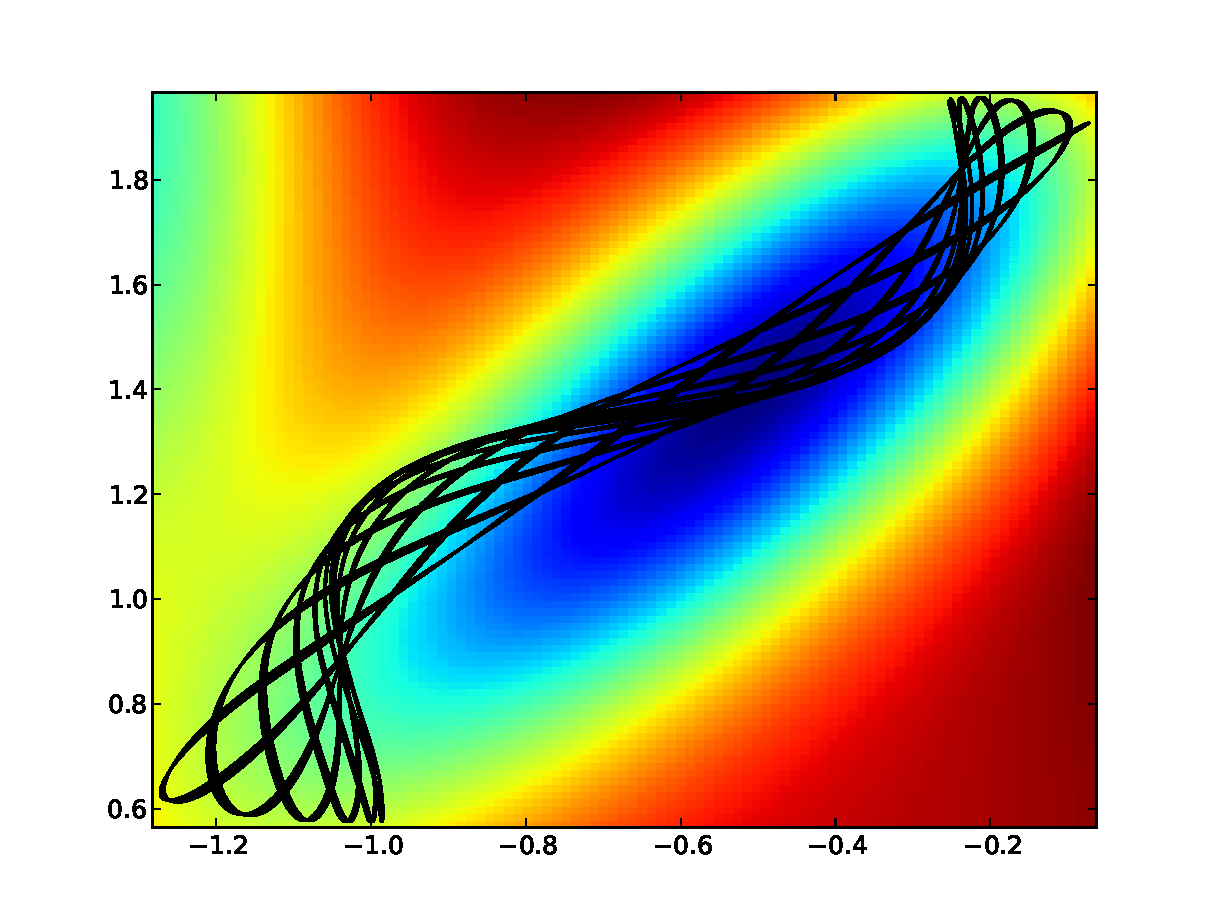
\includegraphics[width=5in]{t6.pdf}
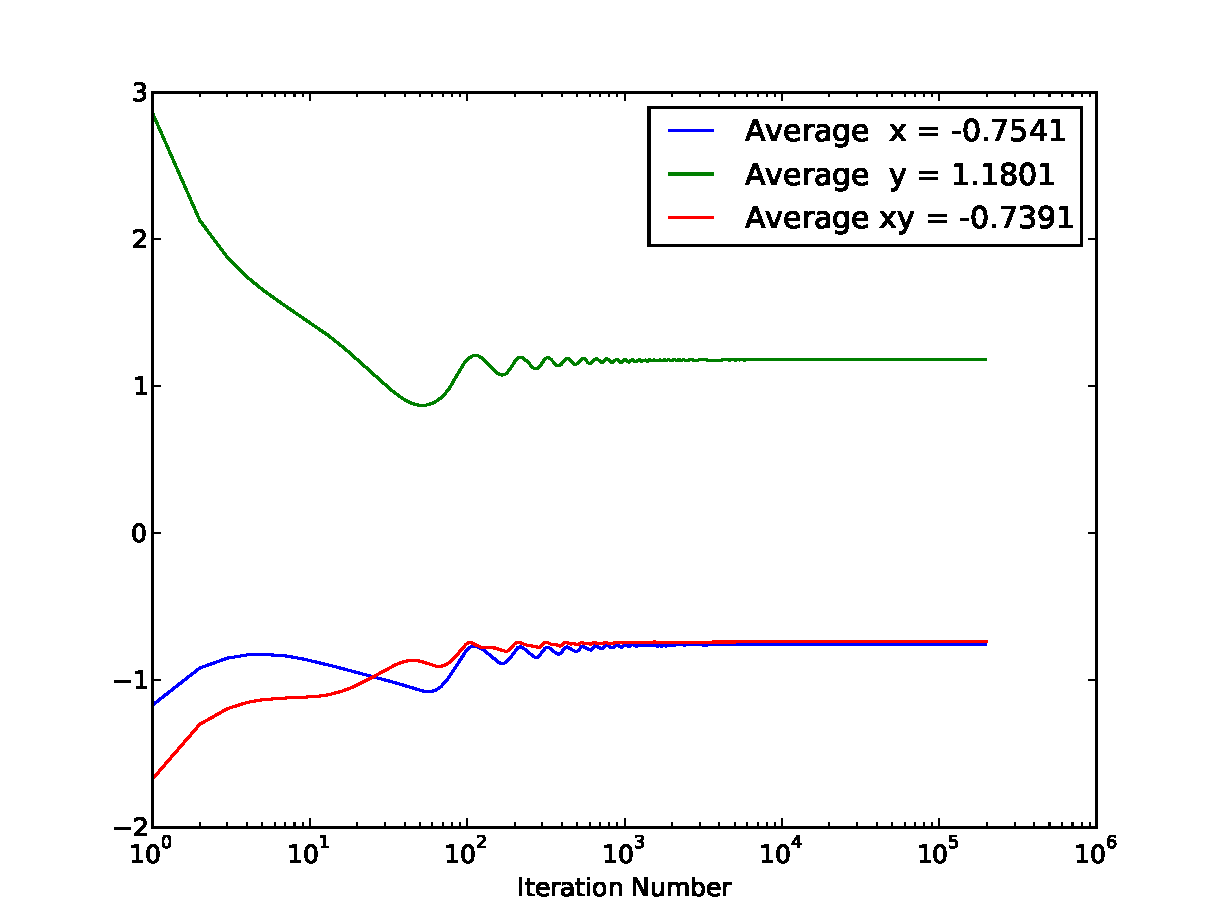
\includegraphics[width=5in]{t6a.pdf}
\end{center}
\caption{$E=-39$: Here is a more extreme case of the previously noted behavior.
Notice the distinctive ribbon path that the particle follows.}
\label{fig:t6}
\end{figure}

\begin{figure}[p]
\begin{center}
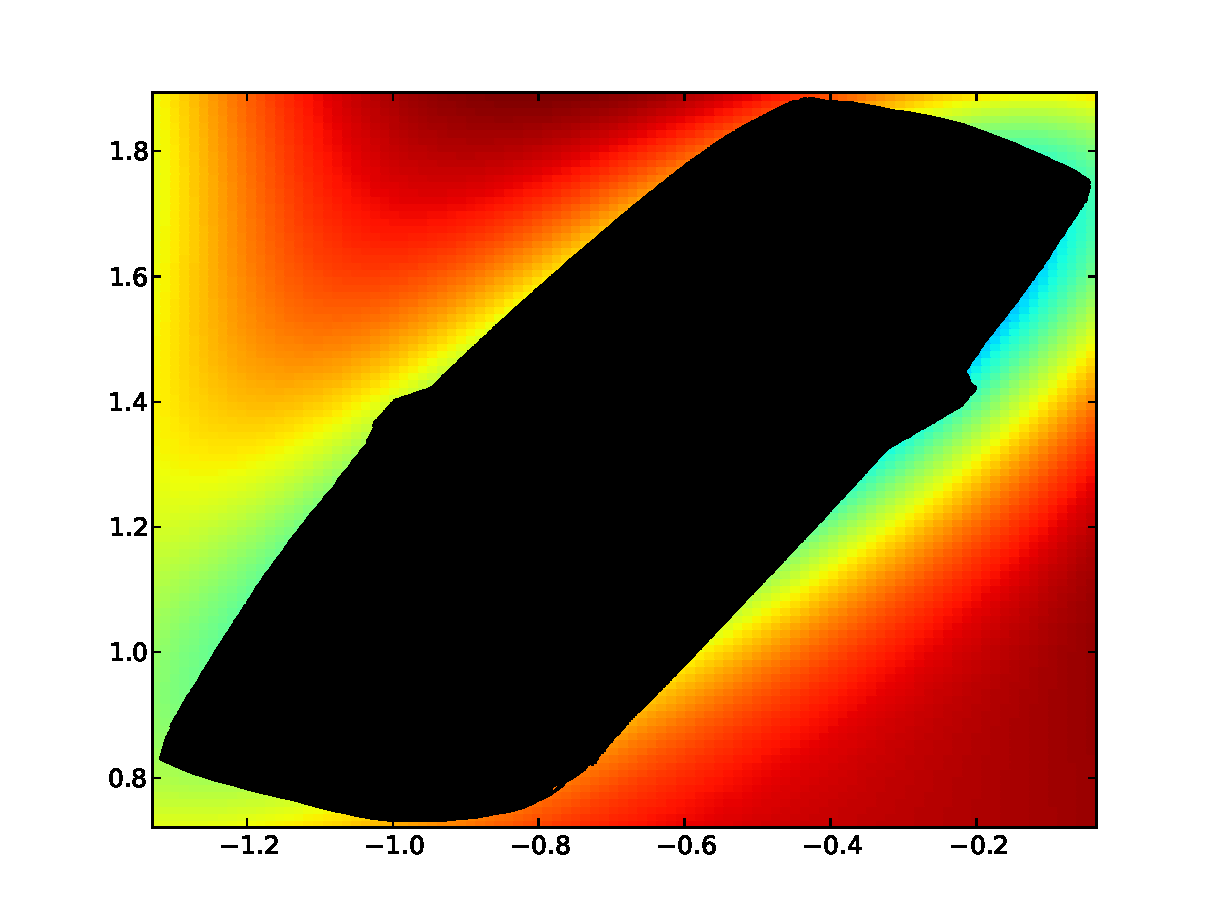
\includegraphics[width=5in]{t7.pdf}
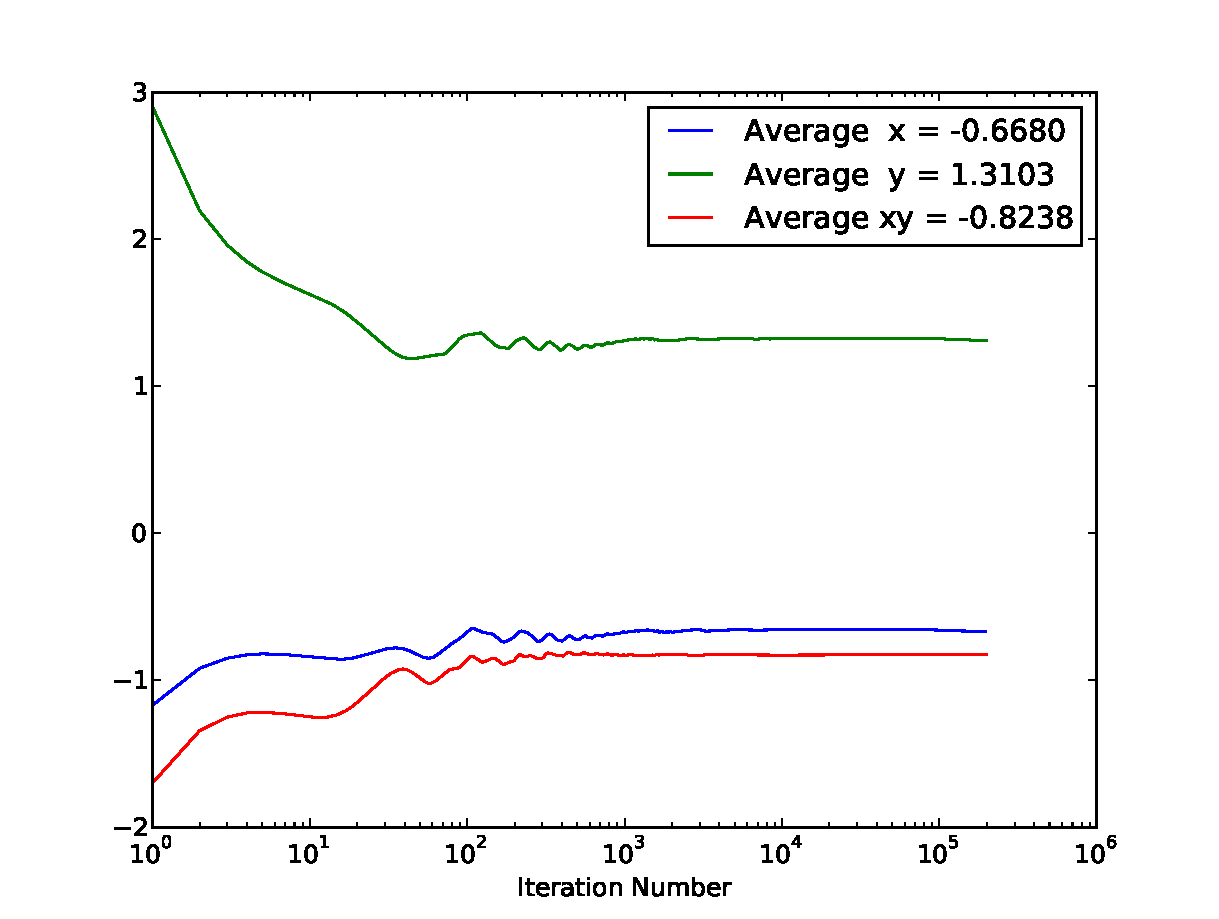
\includegraphics[width=5in]{t7a.pdf}
\end{center}
\caption{$E=-39$: Other times the particle falls into a seemingly random
pattern, but is still never able to leave the well.}
\label{fig:t7}
\end{figure}

\begin{figure}[p]
\begin{center}
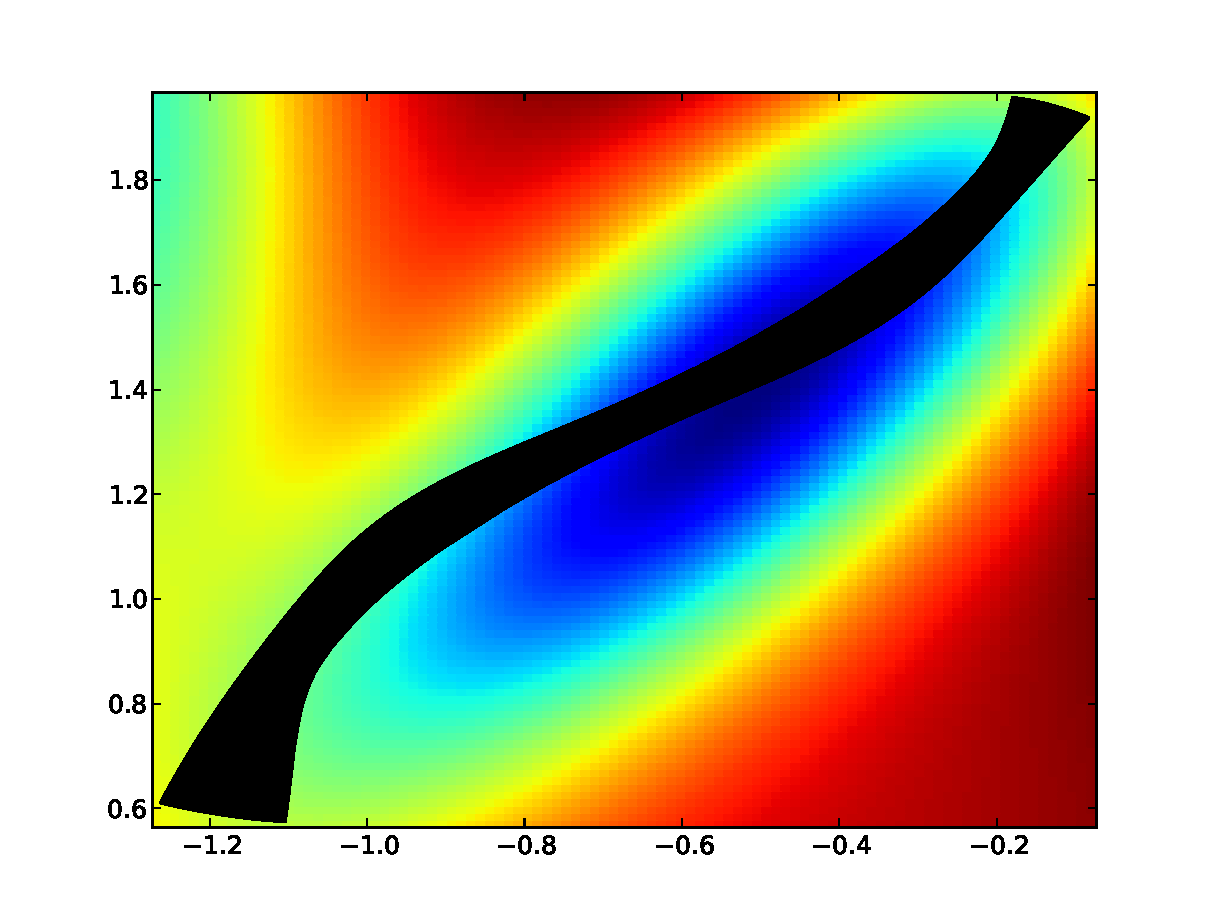
\includegraphics[width=5in]{t4.pdf}
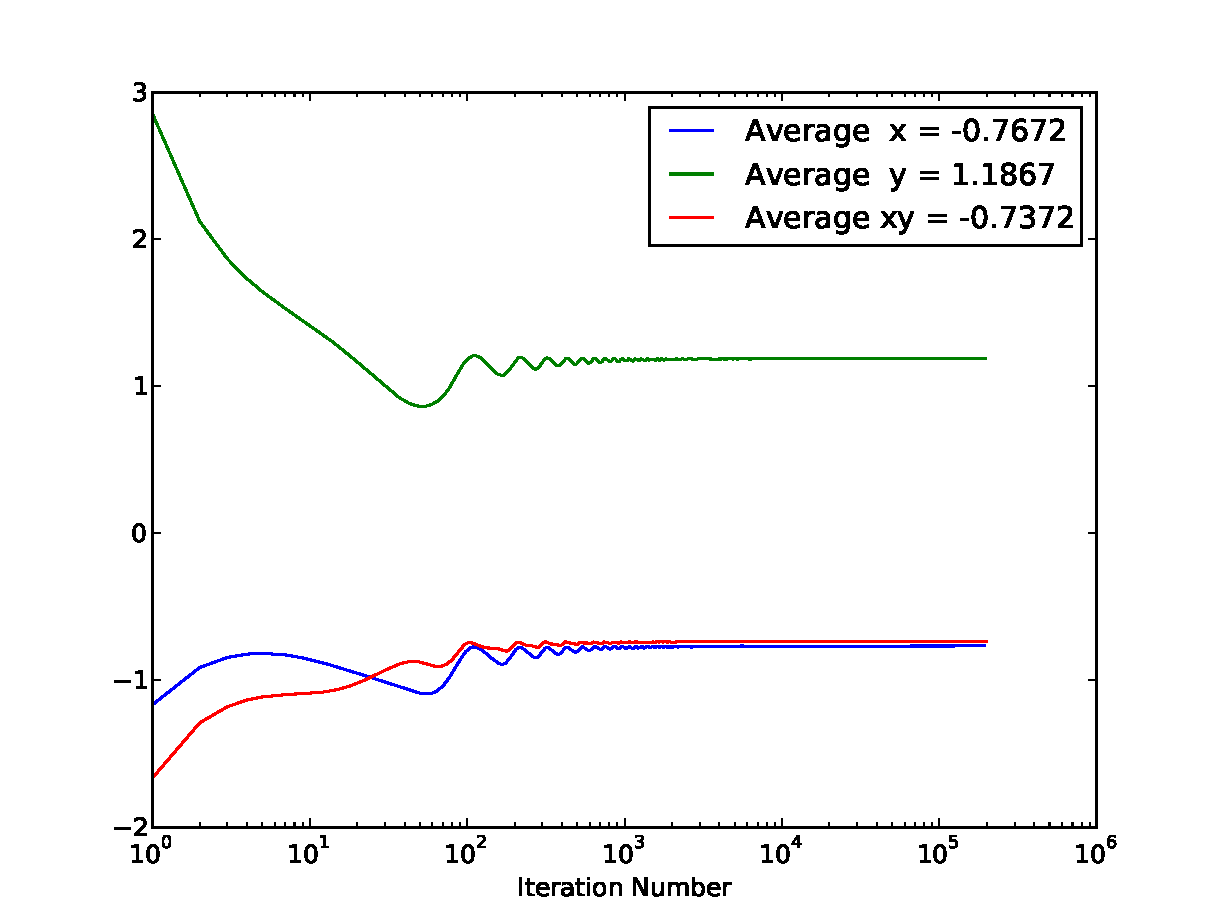
\includegraphics[width=5in]{t4a.pdf}
\end{center}
\caption{$E=-39$: In other cases we get a small ribbon that gets sampled.}
\label{fig:t4}
\end{figure}

\begin{figure}[p]
\begin{center}
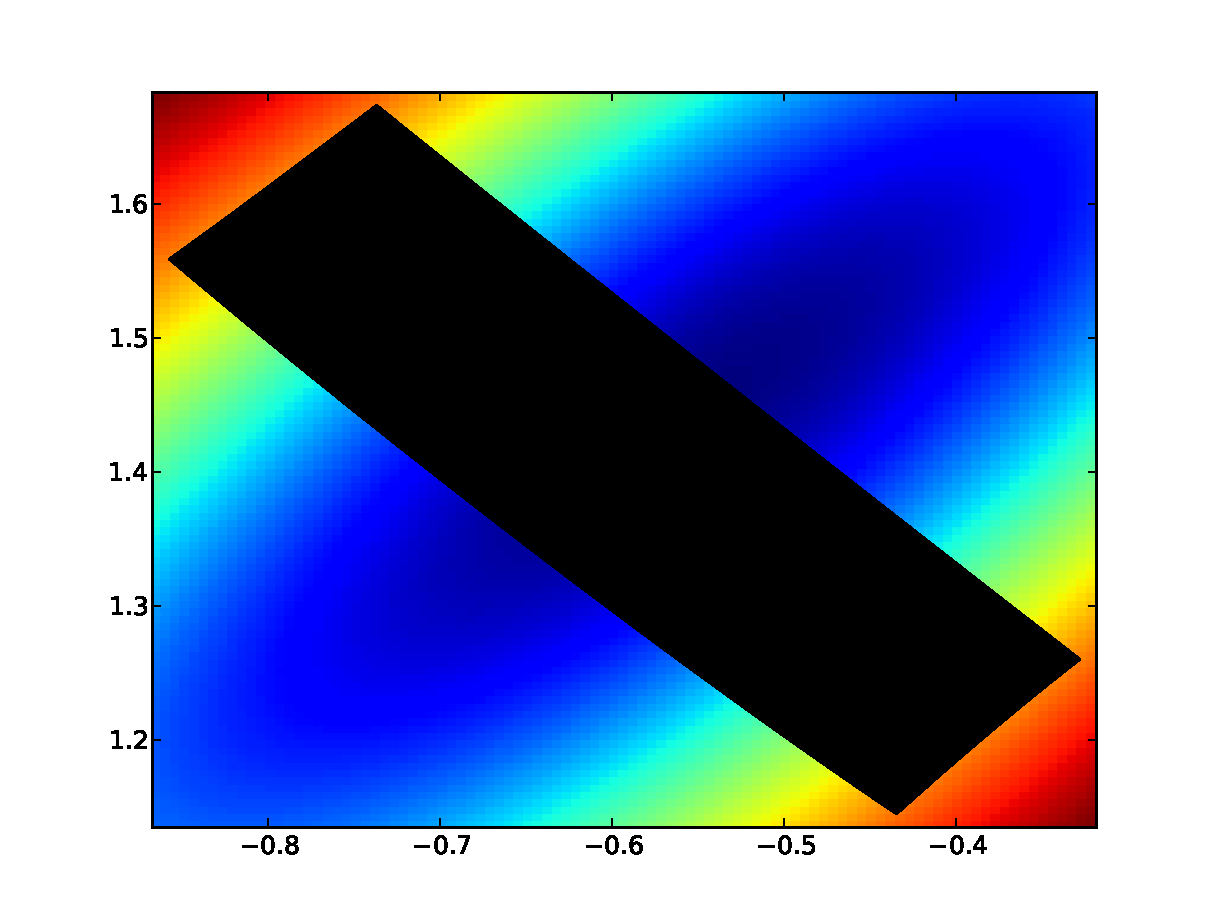
\includegraphics[width=5in]{t3.pdf}
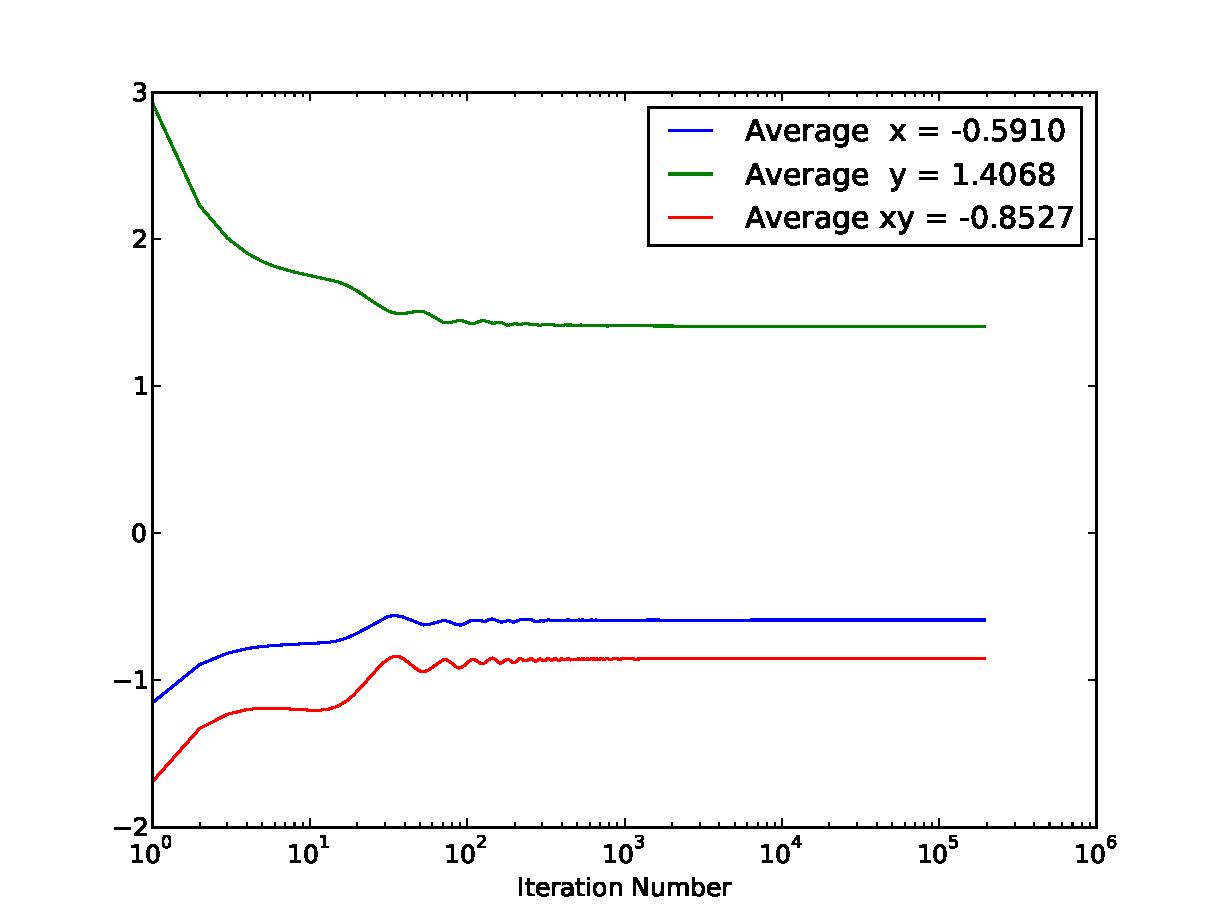
\includegraphics[width=5in]{t3a.pdf}
\end{center}
\caption{$E=-39$: Another common pattern was to get rectangular domains of
sampled points. }
\label{fig:t3}
\end{figure}

\begin{figure}[p]
\begin{center}
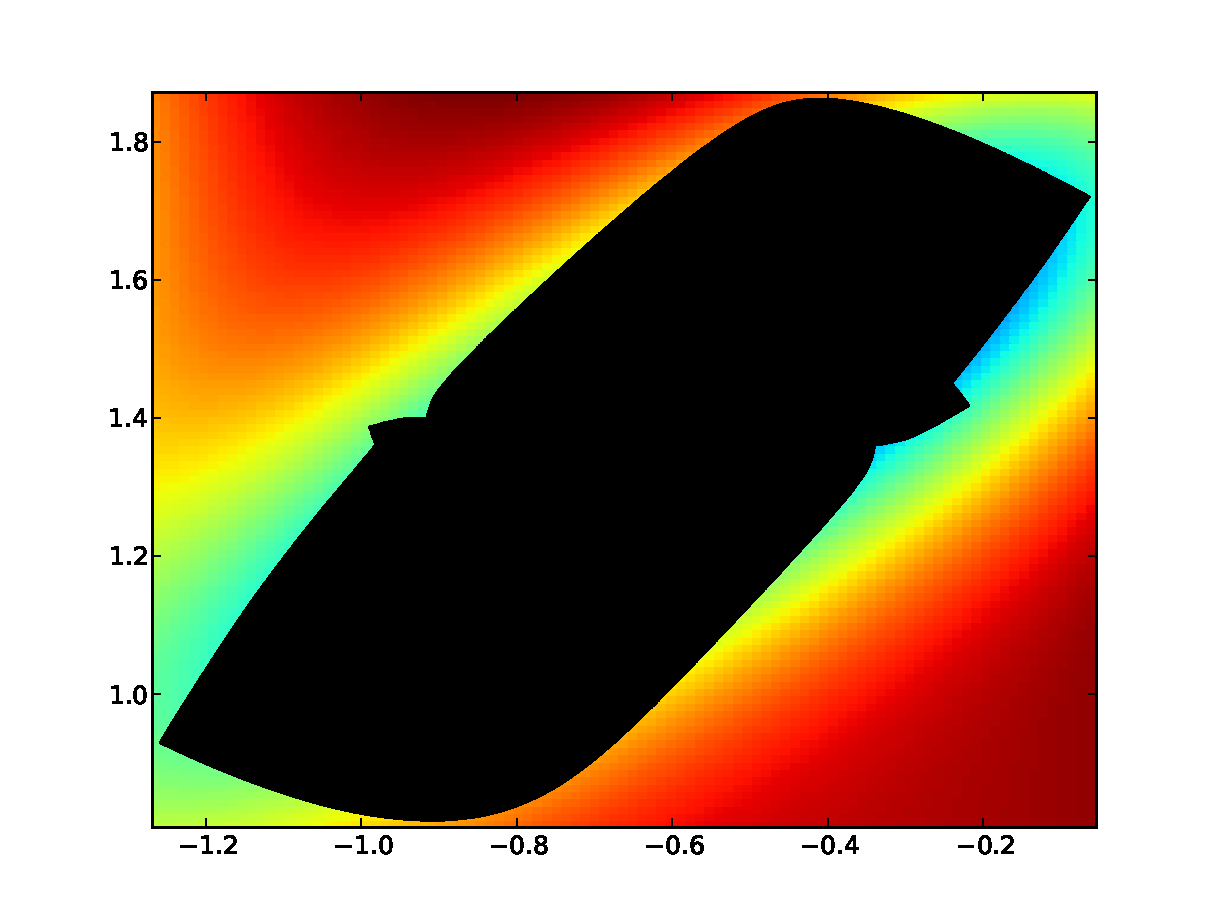
\includegraphics[width=5in]{p5.pdf}
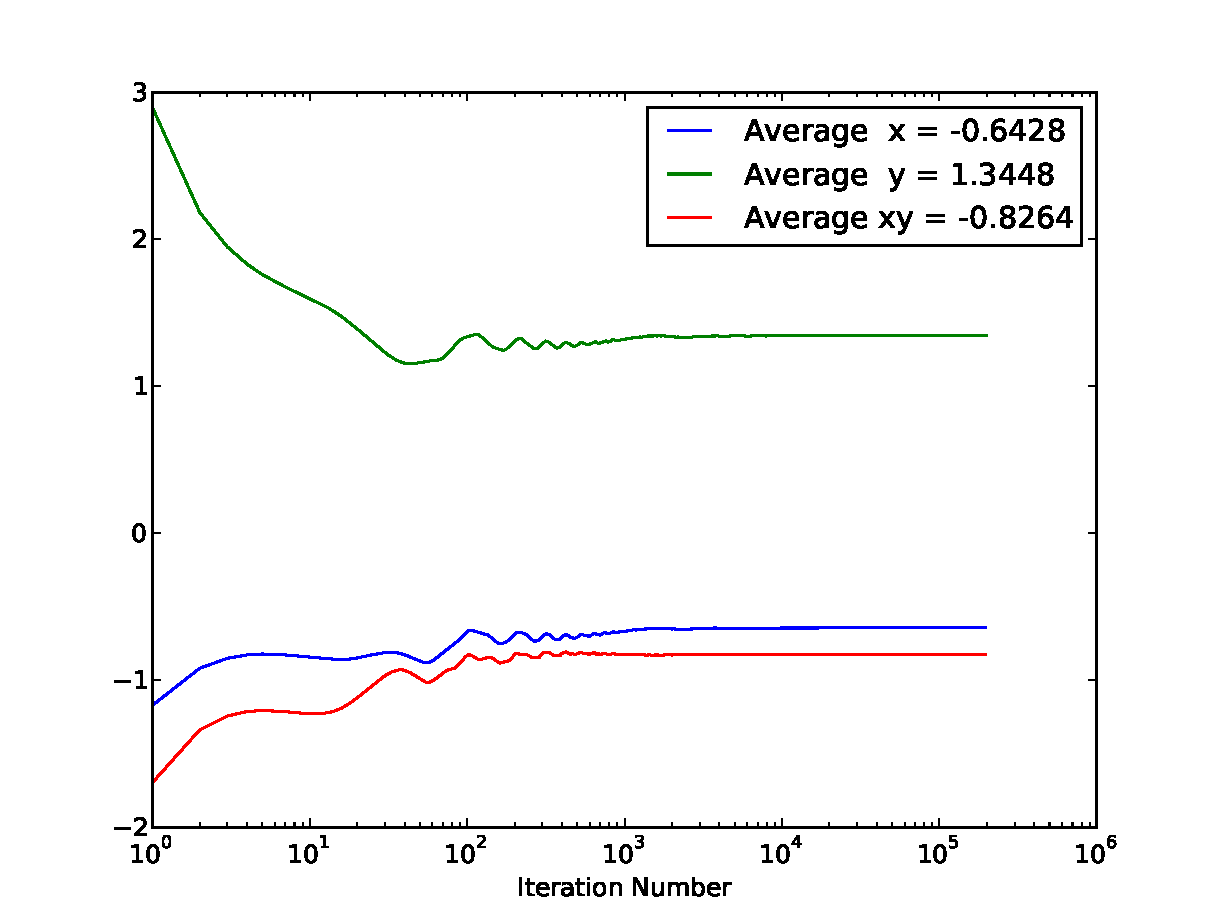
\includegraphics[width=5in]{p5a.pdf}
\end{center}
\caption{$E=-45$: This pattern looks similar to \ref{fig:t7}, except the
particle does not travel as far.}
\label{fig:p5}
\end{figure}

\begin{figure}[p]
\begin{center}
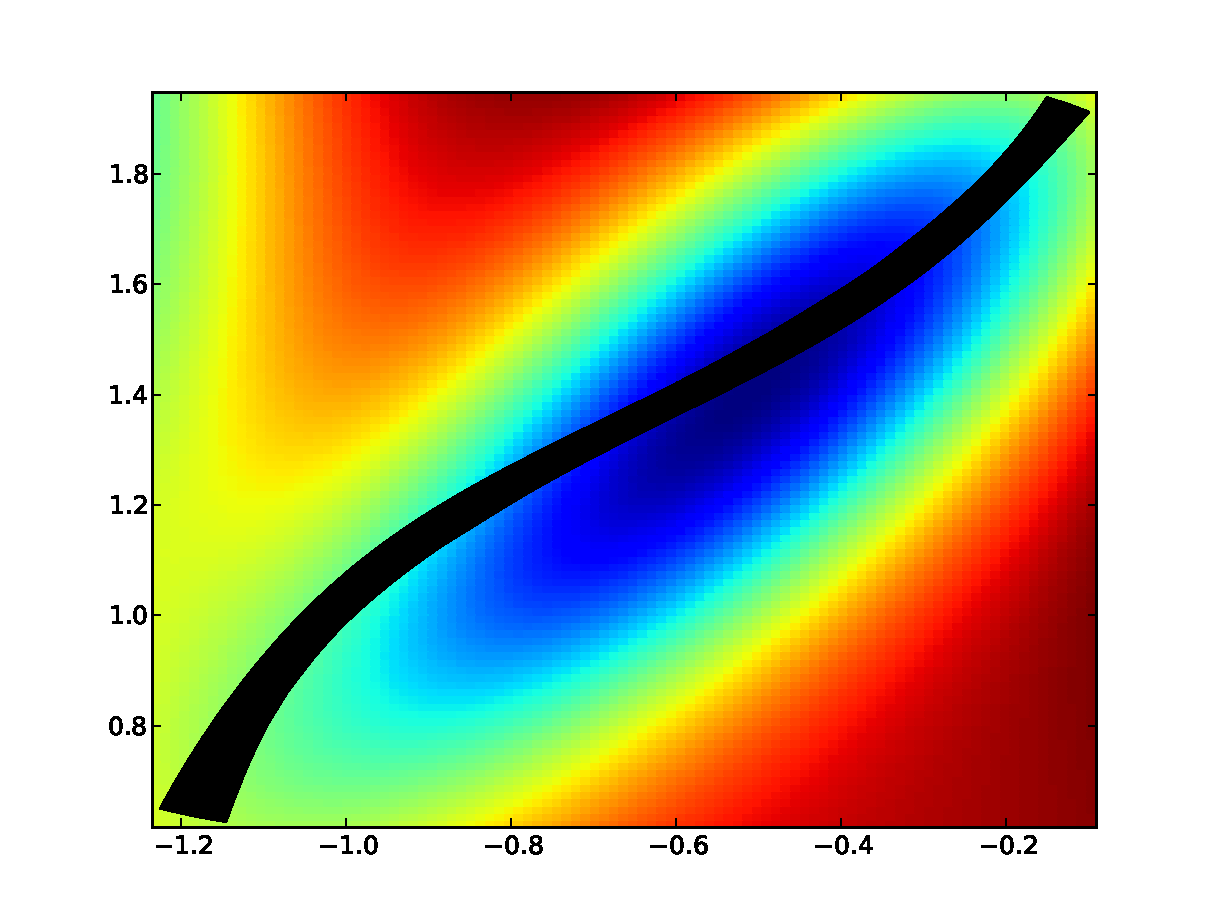
\includegraphics[width=5in]{p3.pdf}
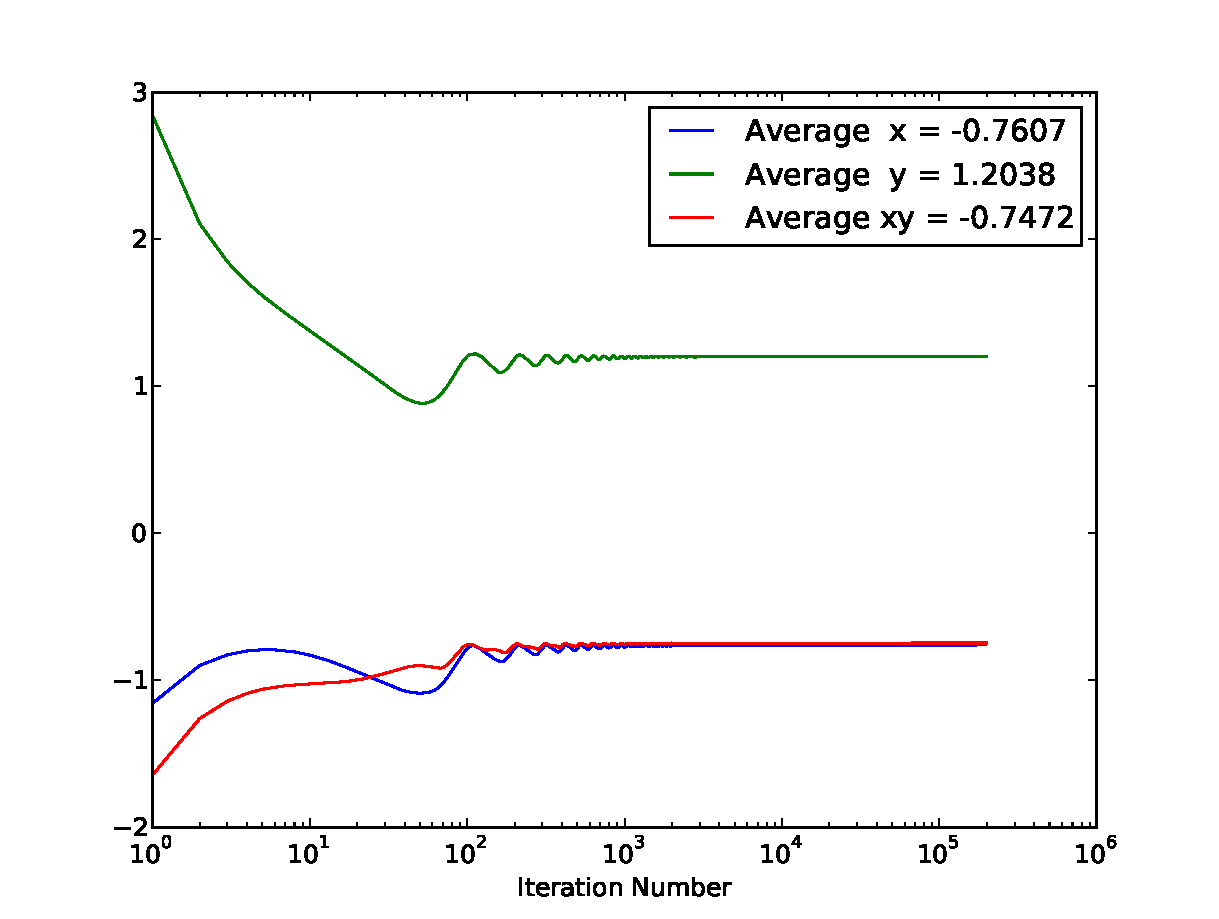
\includegraphics[width=5in]{p3a.pdf}
\end{center}
\caption{$E=-45$: As before, sometimes we get narrow ribbons of sampled points.}
\label{fig:p3}
\end{figure}

\begin{figure}[p]
\begin{center}
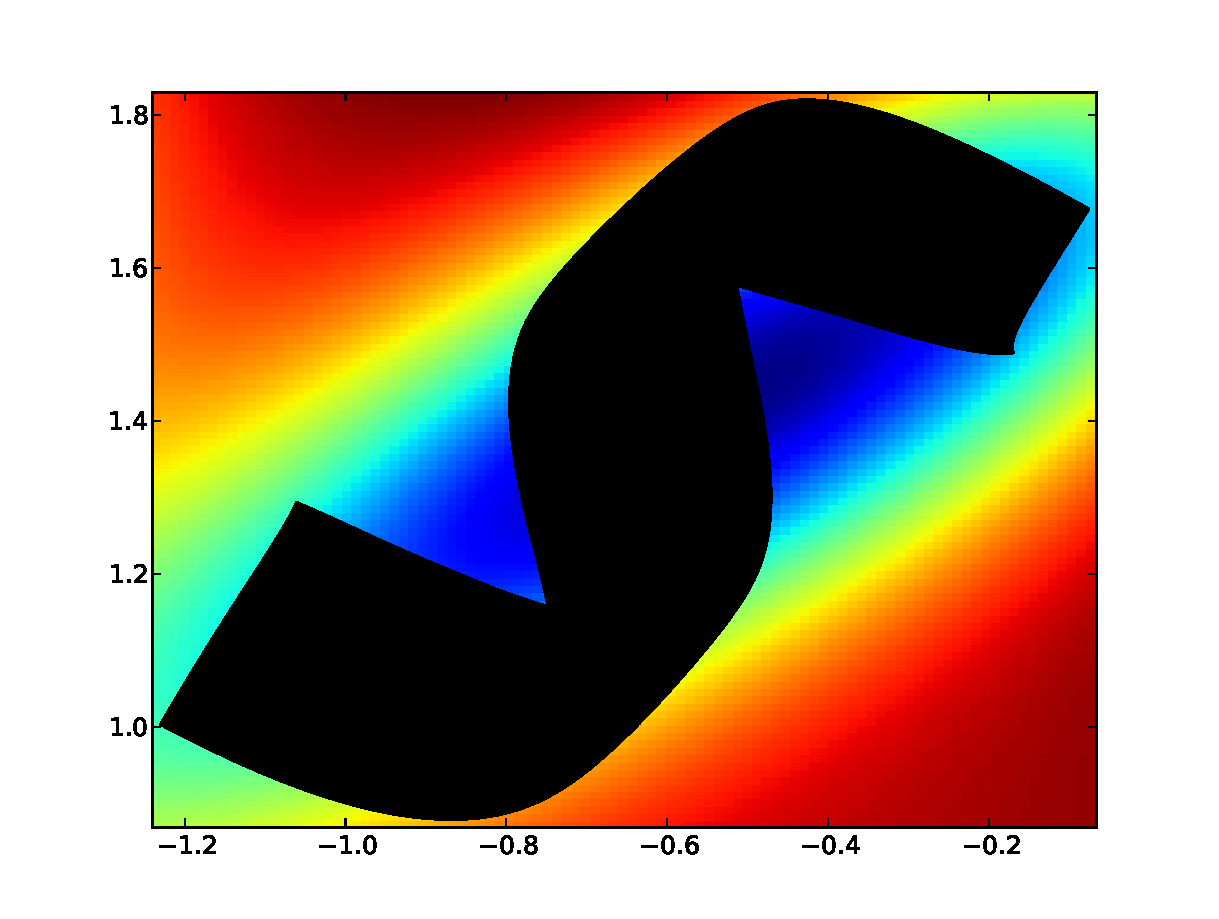
\includegraphics[width=5in]{p4.pdf}
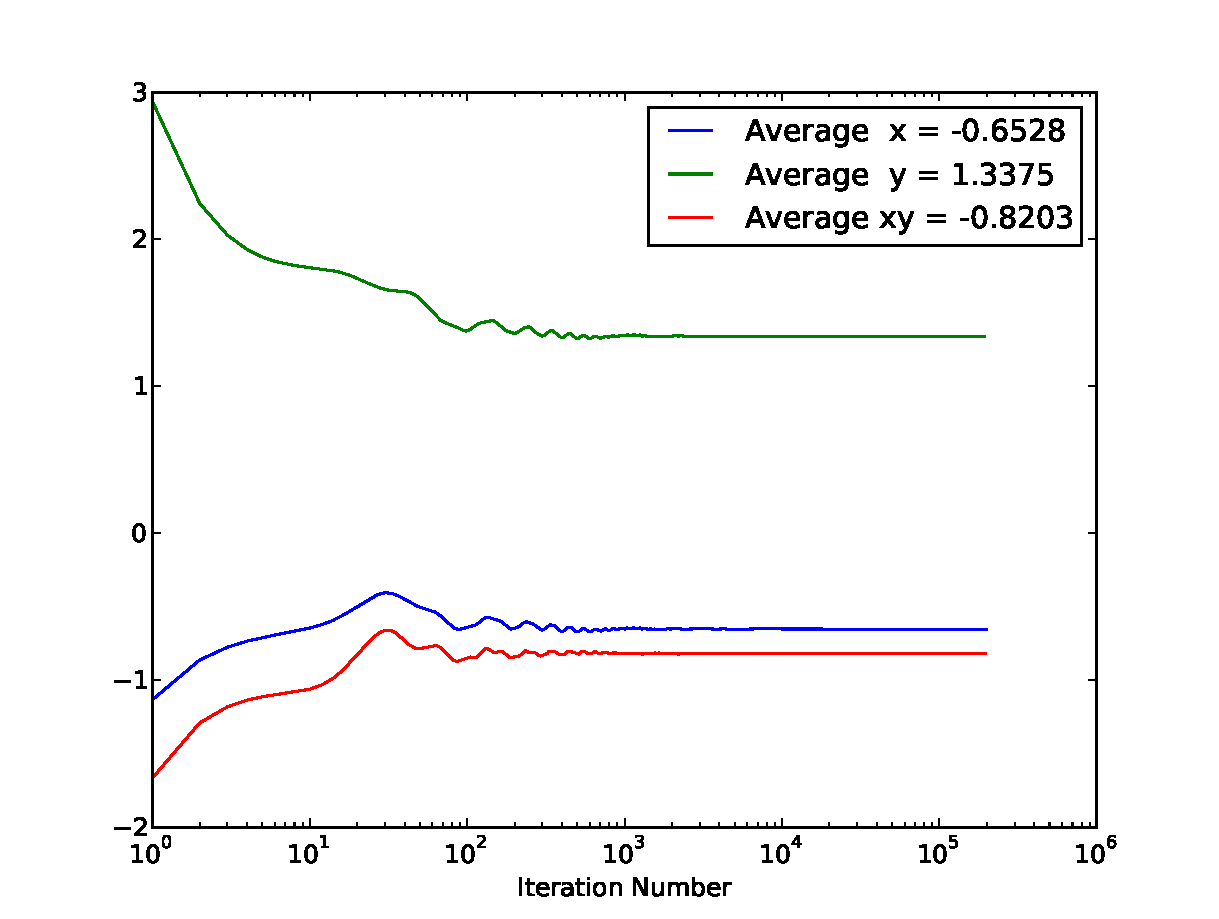
\includegraphics[width=5in]{p4a.pdf}
\end{center}
\caption{$E=-45$: Other times we get S shapes.}
\label{fig:p4}
\end{figure}

\begin{figure}[p]
\begin{center}
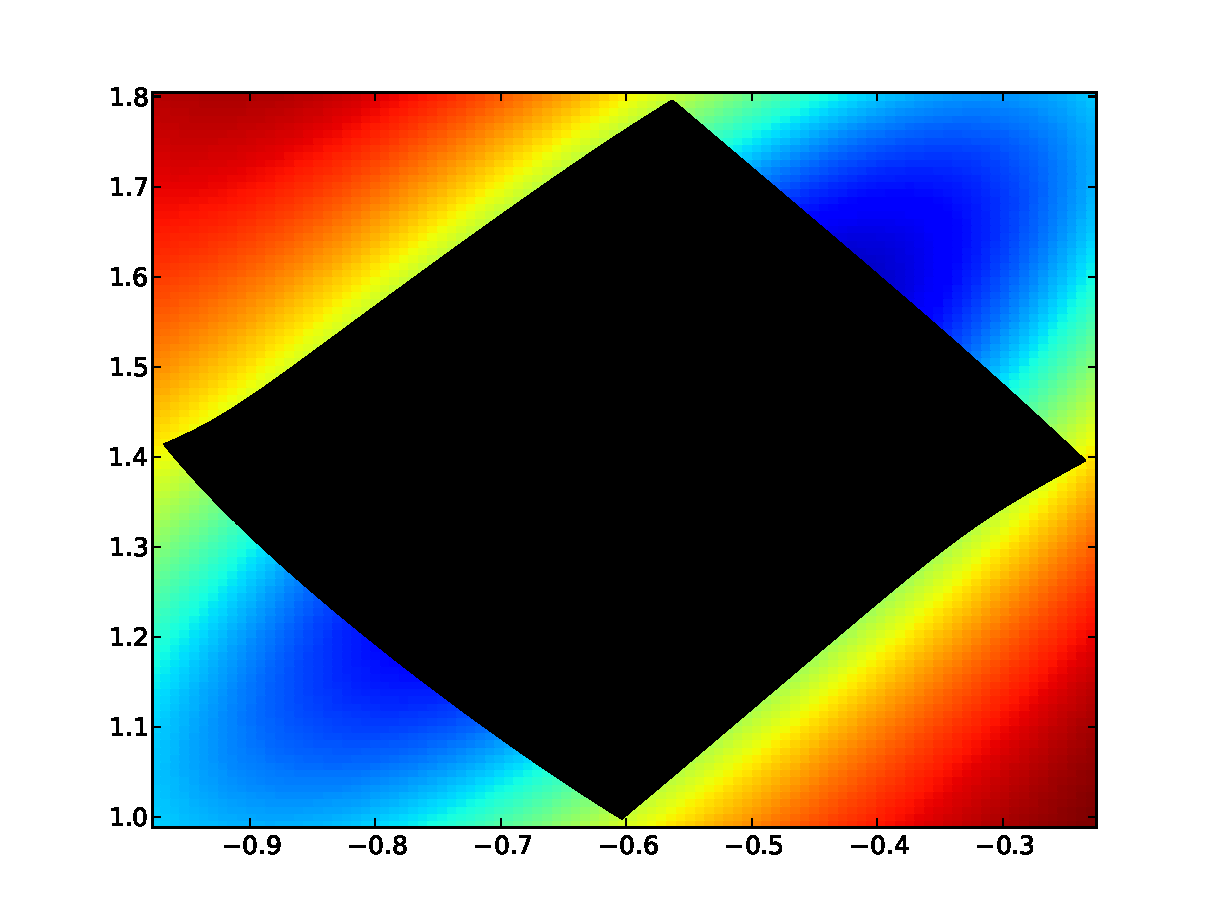
\includegraphics[width=5in]{p1.pdf}
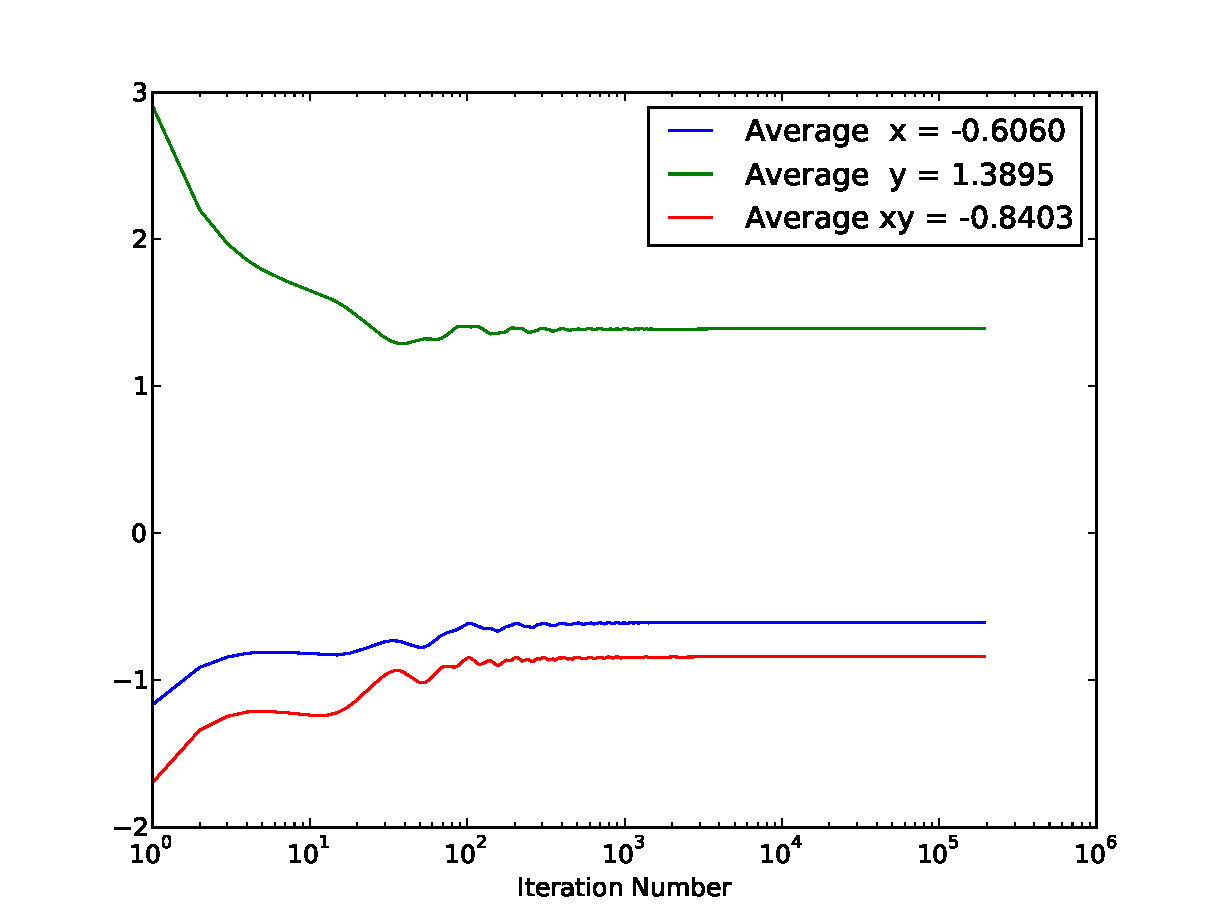
\includegraphics[width=5in]{p1a.pdf}
\end{center}
\caption{$E=-45$: And as before, sometimes we get squares or rectangles.}
\label{fig:p1}
\end{figure}

\newpage 
\clearpage
\lstinputlisting[language=Python,title={HW5.py}]{HW5.py}
\end{document}
